\documentclass{article}
\usepackage{listings}

% Language setting
% Replace `english' with e.g. `spanish' to change the document language
\usepackage[english]{babel}

% Set page size and margins
% Replace `letterpaper' with`a4paper' for UK/EU standard size
\usepackage[letterpaper,top=2cm,bottom=2cm,left=3cm,right=3cm,marginparwidth=1.75cm]{geometry}

% Useful packages
\usepackage{amsmath}
\usepackage{graphicx}
\usepackage[colorlinks=true, allcolors=blue]{hyperref}

\title{Assignment 1}
\author{Owen Bean}

\begin{document}
\maketitle

\section{Code}

\section{Question 1 Response - Zipf's law}

Looking at the graph below of the words vs probability Questions compared to ideal Zipf's law, both graph lines concave up and decreasing. The difference between the two is the Zipf's law is decreasing at a faster rate than the words in questions. For such a small sample size of 171 words, the Question line charactists is similar to Zipf's law. I conclude that the Questions follows expectations of Zip's law.
\\

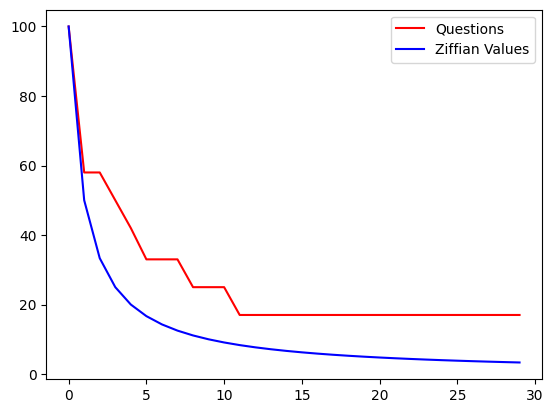
\includegraphics[width=400]{images/zipf.png}

\section{Question 2 Response - Word Cloud}

The most common words including stop words is "the". "the" is the most popular english word. Looking at the word cloud without stop words, "word" is the most frequent word. "word" on the word cloud including stop words looks to be about 50\% of the frequency of "the". This shows there are a decent amount of stop words that is more frequent than "word". Lastly, about half of the top 20 words were stop word. \\ \\

wordCloud with stop words: \hspace*{1.6in} wordCloud without stop words:

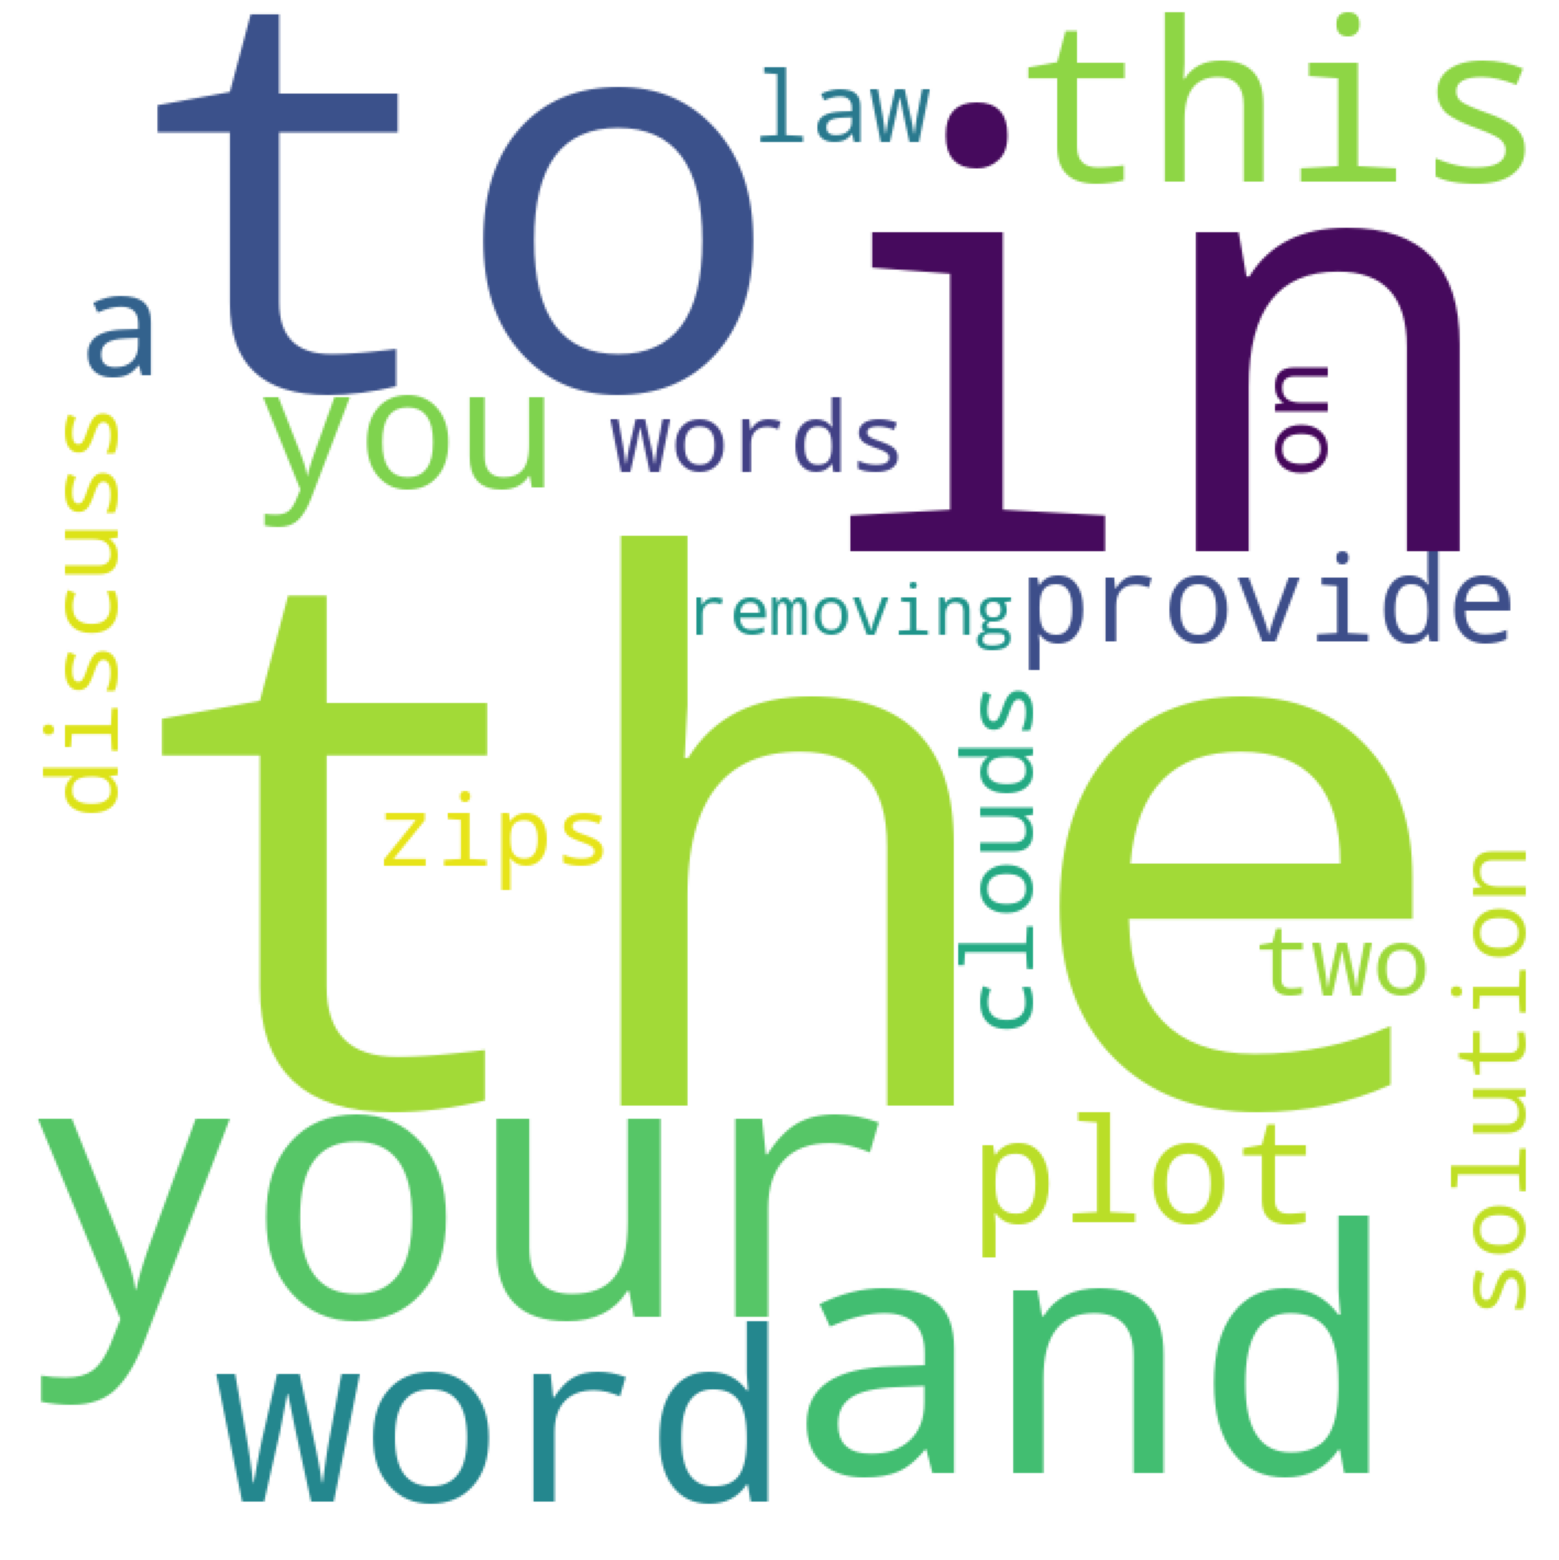
\includegraphics[width=200]{images/wordCloud.png}
\hspace*{0.5in}
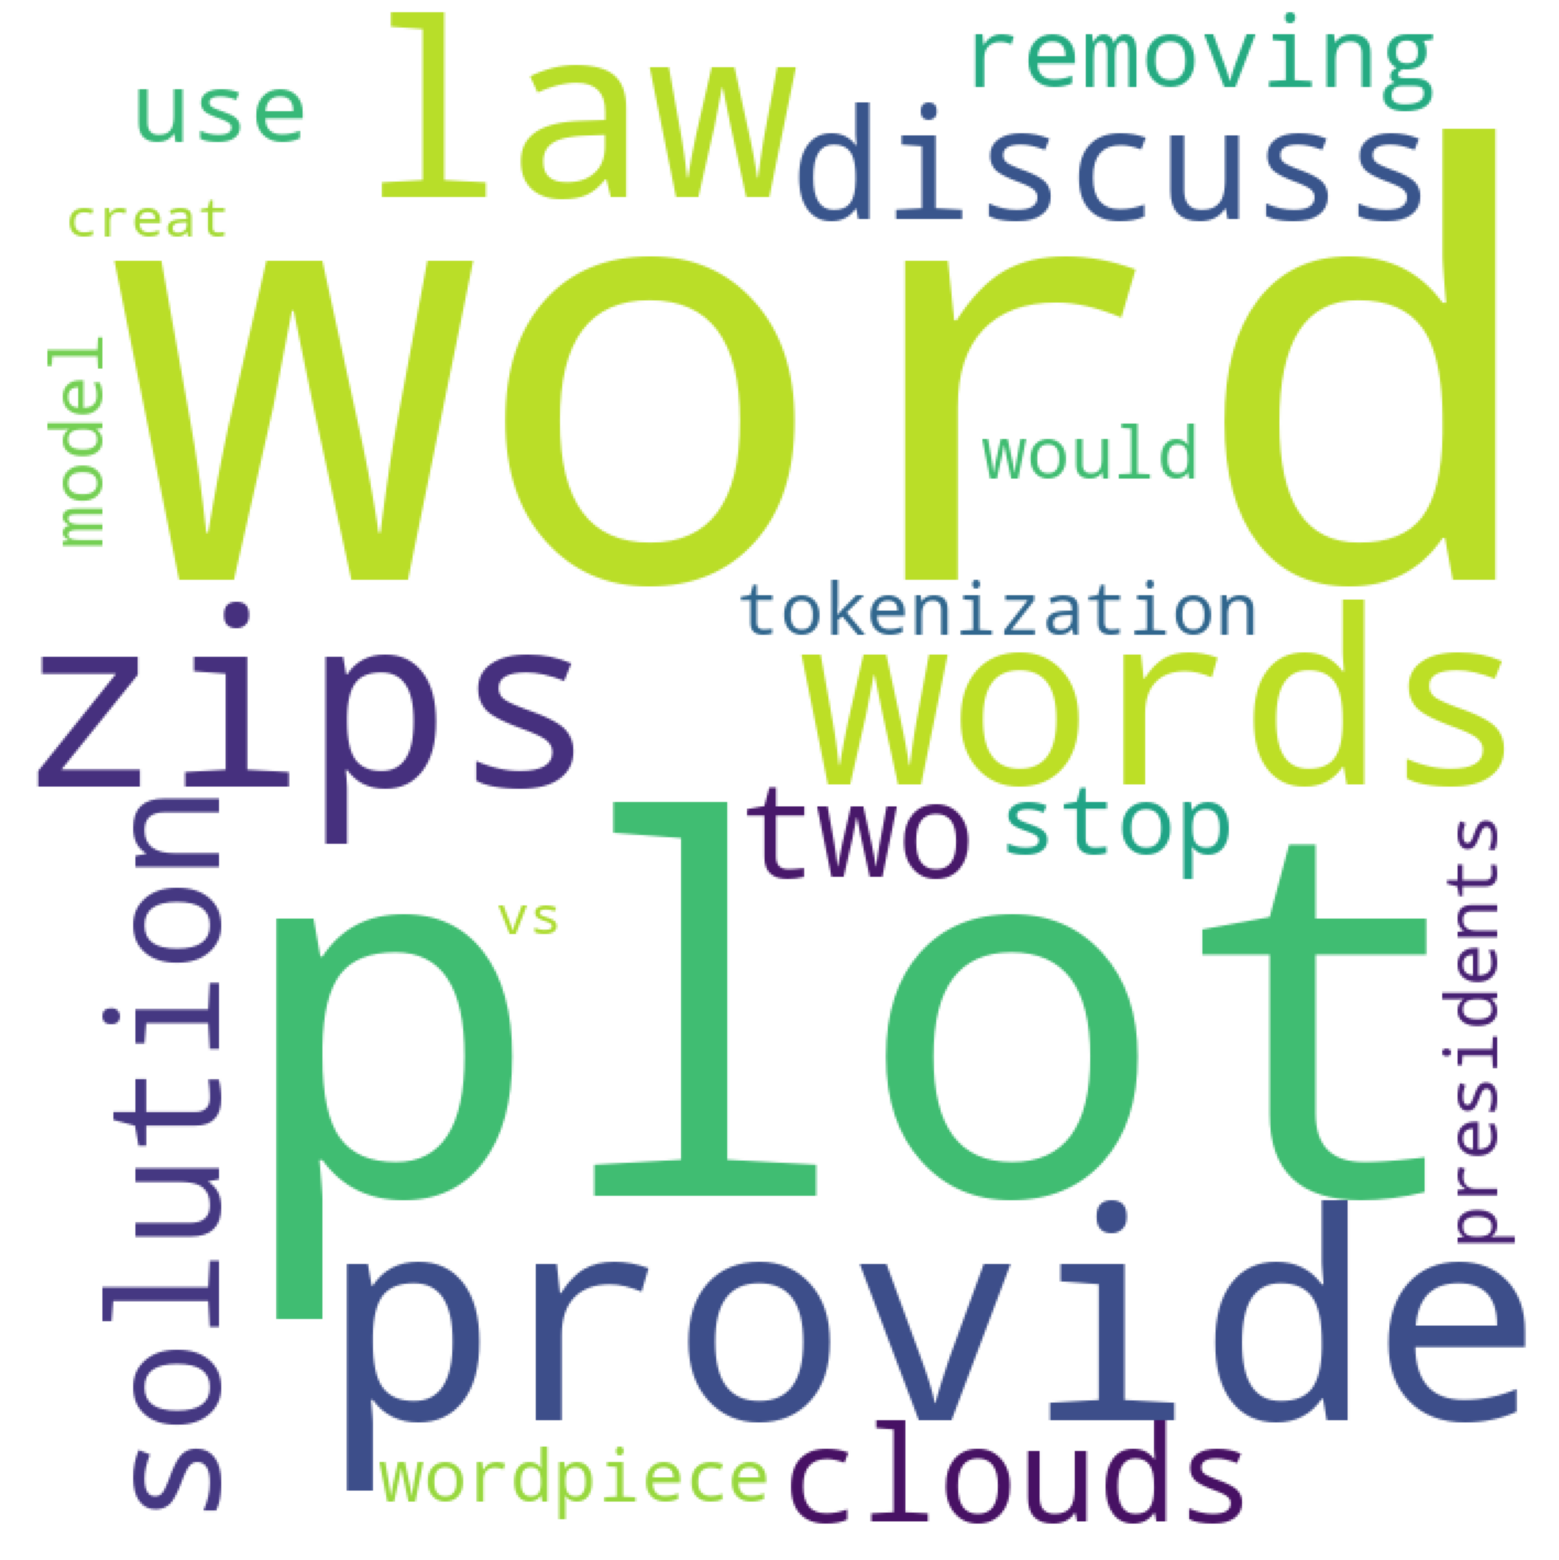
\includegraphics[width=200]{images/wordCloudNoStopWords.png}

\end{document}